\documentclass[10pt]{beamer}

%% Presentation Themes with a Mini Frame Navigation
\usetheme{Frankfurt}  % a variation of Berlin that is slightly less cluttered by leaving out the subsection information
\setbeamertemplate{footline}[page number]
%\usetheme[compress]{Berlin}
%\usetheme{Singapore}

%% Presentation Themes with Section and Subsection Tables
%\usetheme{CambridgeUS}

%% color and font
\usecolortheme{seahorse}
%\usecolortheme{rose}
\usefonttheme{serif}
%\usefonttheme{professionalfonts}

%% special set
\setbeamertemplate{itemize items}[triangle]
\setbeamertemplate{enumerate items}[default]
\setbeamerfont{frametitle}{size=\large}
\setbeamerfont{subsection in toc}{size=\small}

\setbeamertemplate{section in toc}{%
	{\color{blue}\inserttocsectionnumber.}~\inserttocsection}

\setbeamertemplate{subsection in toc}{%
	\hspace{1.5em}{\color{blue}\rule[0.3ex]{3pt}{3pt}}~\inserttocsubsection \par}


\setbeamercovered{transparent}

\setbeamertemplate{footline}[frame number]{}


% both for broad mathematic symbols
\usepackage{amsmath}
\usepackage{amssymb}     
\usepackage{bbm}  % for indicator function
\usepackage{xcolor} % text color


% to change line space
\usepackage{setspace}
%\doublespacing

% enumerate
\usepackage{enumerate}

% input graphs
\usepackage{graphicx}     
% \usepackage{xeCJK}
\graphicspath{ {image/} }

% draw figures
\usepackage{tikz}
\tikzset{
	invisible/.style={opacity=0},
	visible on/.style={alt={#1{}{invisible}}},
	alt/.code args={<#1>#2#3}{%
		\alt<#1>{\pgfkeysalso{#2}}{\pgfkeysalso{#3}} % \pgfkeysalso doesn't change the path
	},
}


% deal with citations
\usepackage{natbib}  
% different citation styles
%\bibliographystyle{unsrtnat}
\bibliographystyle{apalike}


% make tables
\usepackage{threeparttable, booktabs}
\usepackage{adjustbox}
\usepackage{booktabs}

% place tables in the exact page I want, uisng \FloatBarrier
\usepackage{placeins}    

% hyperlinks
\usepackage{hyperref} 

\usepackage{appendixnumberbeamer} 



\begin{document}
	\setbeamertemplate{navigation symbols}{}
	% turn off navigation symbols at the the bottom right-hand corner of the screen



%%%%%%%%%%%%%%%%%%%%%%%%%%%
\begin{frame}[shrink=40]{Model Predictions}
\begin{figure}
	\centering
	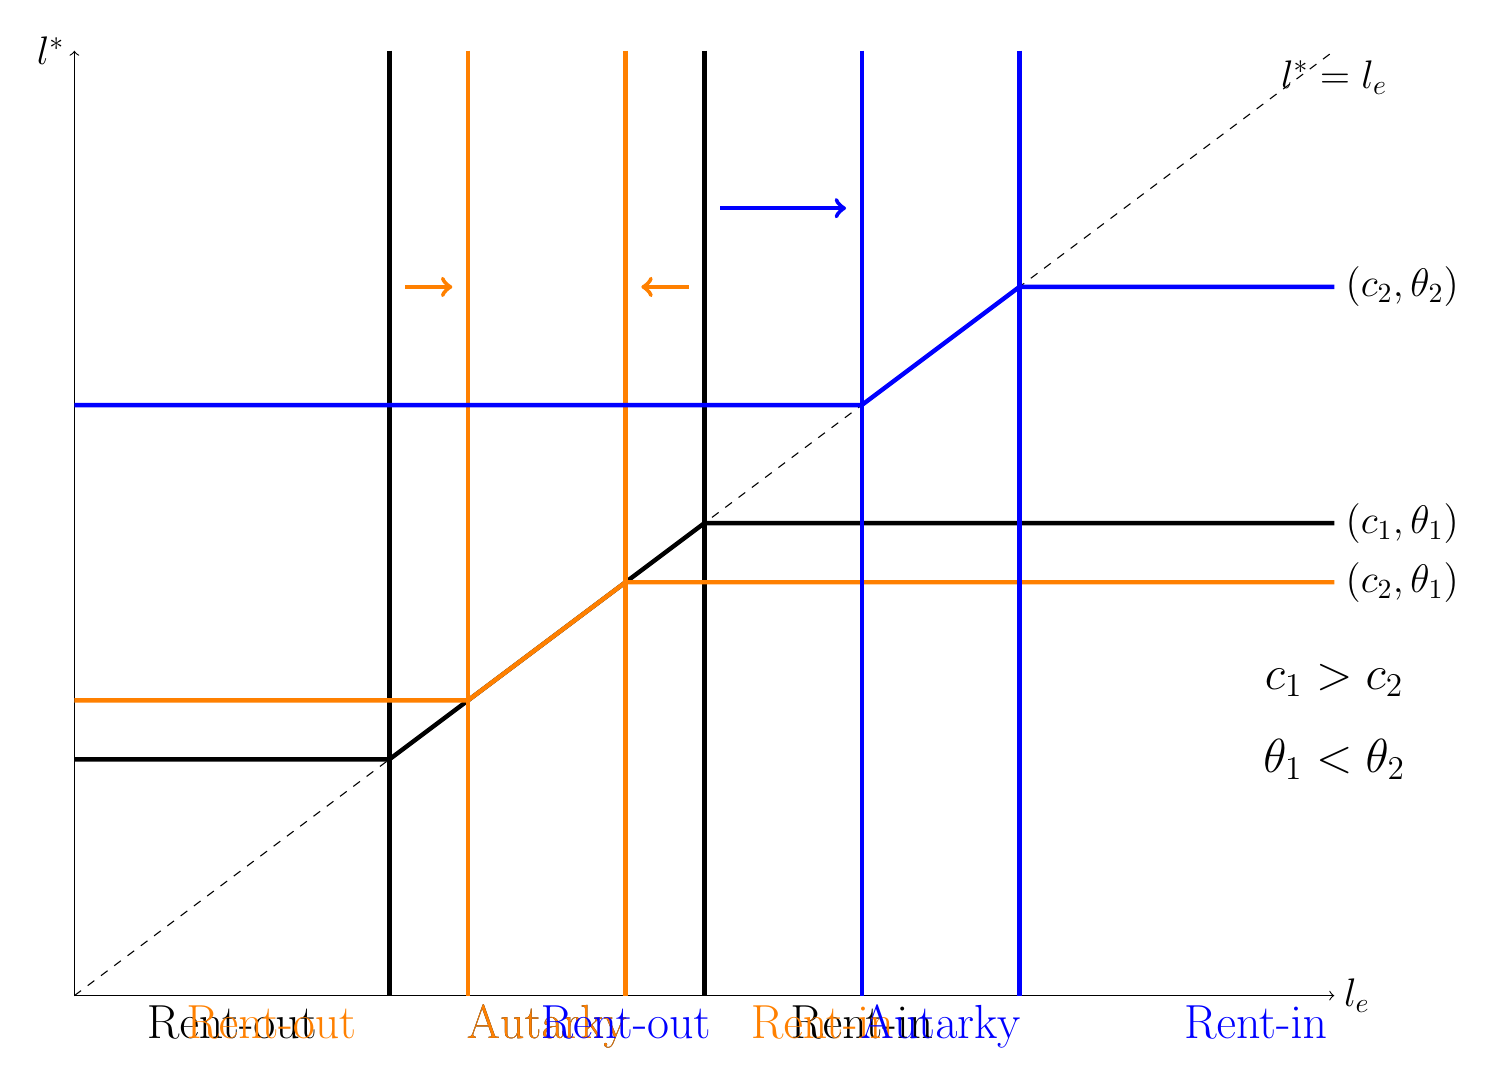
\begin{tikzpicture}
	% setup
	\draw [->, visible on=<1->] (0,0) - - (16,0) node[right]{\Large $l_e$};
	\draw [->, visible on=<1->] (0,0) - - (0,12) node[left]{\Large $l^*$};
	\draw [dashed, visible on=<1->] (0,0) -- (16, 12) node[below]{\Large $l^*=l_e$};
	
	% original optimization
	\draw [ultra thick, visible on=<1->] (4,12) -- (4,0);
	\draw [ultra thick, visible on=<1->] (8,12) -- (8,0);
	\draw [ultra thick, visible on=<1->] (0,3) -- (4,3)--(8,6)--(16,6) node[right,black]{\Large $(c_1,\theta_1)$} ;
	\node [below, visible on=<1>] at (2,0) {\LARGE Rent-out};
	\node [below, visible on=<1>] at (6,0) {\LARGE Autarky};
	\node [below, visible on=<1>] at (10,0) {\LARGE Rent-in};
	
	% new optimization, change c given theta
	\draw [ultra thick, orange, visible on=<2->] (5,12) -- (5,0);
	\draw [ultra thick, orange, visible on=<2->] (7,12) -- (7,0);
	\draw [ultra thick, orange, visible on=<2->] (0,3.75) -- (5,3.75)--(7,5.25)--(16,5.25) node[right, black]{\Large $(c_2, \theta_1)$};
	\draw [->, ultra thick, orange, visible on=<2->] (4.2,9) -- (4.8, 9);
	\draw [->, ultra thick, orange, visible on=<2->] (7.8,9) -- (7.2, 9);
	\node [below, visible on=<2>, orange] at (2.5,0) {\LARGE Rent-out};
	\node [below, visible on=<2>, orange] at (6,0) {\LARGE Autarky};
	\node [below, visible on=<2>, orange] at (9.5,0) {\LARGE Rent-in};
	
	% new optimization, change both c and theta
	\draw [ultra thick, blue, visible on=<3->] (10,12) -- (10,0);
	\draw [ultra thick, blue, visible on=<3->] (12,12) -- (12,0);
	\draw [ultra thick, blue, visible on=<3->] (0,7.5) -- (10,7.5)--(12,9)--(16,9) node[right, black]{\Large $(c_2,\theta_2)$};
	\draw [->, ultra thick, blue, visible on=<3->] (8.2,10) -- (9.8, 10);
	\node [below, visible on=<3>, blue] at (7,0) {\LARGE Rent-out};
	\node [below, visible on=<3>, blue] at (11,0) {\LARGE Autarky};
	\node [below, visible on=<3>, blue] at (15,0) {\LARGE Rent-in};	
	
	% legend
	\node [visible on=<2->] at (16,4) {\LARGE $c_1 > c_2$};			
	\node [visible on=<3->] at (16,3) {\LARGE $\theta_1 < \theta_2$};
	\end{tikzpicture}
\end{figure}
\end{frame}

\end{document}